\documentclass{letter}

\usepackage[utf8]{inputenc}
\usepackage[T1]{fontenc}
\usepackage{hyperref}
\usepackage{graphicx}
\usepackage{fancyhdr}
\usepackage{geometry}

\usepackage{fancyhdr}
\usepackage[usenames,dvipsnames,svgnames]{xcolor}

\pagestyle{fancy}
\lhead{}
\rhead{}
\chead{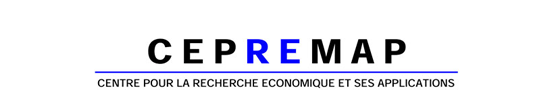
\includegraphics[scale=.35]{../img/cepremap.png}\\ {\footnotesize \textbf{\textcolor{CornflowerBlue}{DYNARE Summer School (Banque de France)}}}\\ {\footnotesize \textbf{\textcolor{CornflowerBlue}{June 11th, 2018 – June 15th, 2018}}}}
\lfoot{}
\rfoot{}
\cfoot{}

\renewcommand{\footrulewidth}{0pt}
\renewcommand{\headrulewidth}{0pt}

\address{CEPREMAP/ENS\\ 48 Boulevard Jourdan\\ 75014 Paris, France}

\begin{document}

\begin{letter}{}
  
  \bigskip
  \bigskip
  \bigskip
  
\opening{To whom it may concern,}

\thispagestyle{fancy}

  \bigskip
  \bigskip
  \bigskip

We are pleased to inform you that :{FIRSTNAME}: :{LASTNAME}: has been accepted in the Dynare Summer School that will take place from June 11th to June 15th 2018 at Banque de France (Paris, France). The registration fee for the week (courses, coffee breaks, lunches and one diner included) is 200€.

  \bigskip
  \bigskip
  \bigskip
  \bigskip
  \bigskip
  \bigskip
  \bigskip
  
\closing{Best regards,\\
\fromsig{\includegraphics[scale=.04]{../img/signature.jpg}} \\
\fromname{Stéphane Adjemian\\In charge of the Dynare project}
}

\end{letter}
\end{document}
